%! TEX program = pdflatex
%% Mauricio Caceres Bravo <mauricio.caceres.bravo@gmail.com>

%----------------------------------------------------------------------
\documentclass{article}

\usepackage[summary]{brownpreamble}
\usepackage{etoc}
\setcounter{tocdepth}{3}

\renewcommand{\subsectionmark}[1]{\markboth{#1}{}}
\renewcommand\sectiontype{Lecture \thesection:\ }
\lhead{\color{light-gray} \itshape Math Camp Aug 23, 2022 -- Lecture \thesection}
\rhead{\color{light-gray} \itshape \thesubsection. \leftmark}
\setcounter{section}{5}
% \renewcommand\SetHideLevel{1pt}
% TODO: xx add spectral decomposition and some eigenstuff related to PD/ND

%----------------------------------------------------------------------
\begin{document}
\displayoptions

% ---------------------------------------------------------------------
\section{Linear Algebra, ODE and Dynamic Systems}
\label{sec:linear_algebra_ode_and_dynamic_systems}

\localtableofcontents

% ---------------------------------------------------------------------
\subsection{Linear Algebra}
\label{sub:linear_algebra}

% Lecture 6:
%     Intro
%     Vector spaces
%     Linear combinations
%     Remark that in fact a more abstract theory using generic linear spaces leads you to a theorem that all linear spaces are isomorphic  to R^N for all linear algebra purposes.
%     Matrix inversion
%     Mention linear algebra hand-out and how you transcribed it (MAHO?).
%     characteristic polynomial, eigenvalues, misc foo from Oded and MAHO
%     trace and trace tricks from MAHO
%     "Spectral theorem" (matrix diagonaization)

In economics, it is very common to have \keyword{systems of equations},
\begin{equation}
  \begin{array}{rl}
    Q_d & = a_0 + a_1 P \\
    Q_s & = b_0 + b_1 P \\
    Q_d  - Q_s & = 0
  \end{array}
  \label{eq:lecture6_supply_demand}
\end{equation}

We have supply, demand, and equilibrium. This is oozing economics, right? This problem can be expressed in general as
\begin{align*}
  A x = d
\end{align*}

with $A$ some $N \times M$ matrix times a column vector $x \in \mathbb{R}^M$ equal to some other vector $d \in \mathbb{R}^N$. The above is matrix notation for the system
\begin{equation}
  \begin{array}{rl}
    a_{11} x_1 = a_{12} x_2 + \ldots + a_{1M} x_M & = d_1 \\
    \vdots \\
    a_{N1} x_1 = a_{N2} x_2 + \ldots + a_{NM} x_M & = d_N
  \end{array}
  \nonumber
\end{equation}

With some wrangling, we can see that \Cref{eq:lecture6_supply_demand} can be expressed in this way:
\begin{align*}
  \underbrace{
    \begin{bmatrix}
      a_0
      \\
      b_0
      \\
      0
    \end{bmatrix}
  }_{d}
  &
  =
  \underbrace{
    \begin{bmatrix}
      - a_1 & 1 & 0
      \\
      - b_1 & 0 & 1
      \\
      0 & 1 & -1
    \end{bmatrix}
  }_{A}
  \underbrace{
    \begin{bmatrix}
      P
      \\
      Q_d
      \\
      Q_s
    \end{bmatrix}
  }_{x}
\end{align*}

In this case, $A$ is $3 \times 3$ and ``invertible,'' so we can explicitly solve for equilibrium price and quantity.
\begin{align*}
  \begin{bmatrix}
    P
    \\
    Q_d
    \\
    Q_s
  \end{bmatrix}
  &
  =
  \begin{bmatrix}
    - a_1 & 1 & 0
    \\
    - b_1 & 0 & 1
    \\
    0 & 1 & -1
  \end{bmatrix}^{-1}
  \begin{bmatrix}
    a_0
    \\
    b_0
    \\
    0
  \end{bmatrix}
  \\
  \begin{bmatrix}
    P
    \\
    Q_d
    \\
    Q_s
  \end{bmatrix}
  &
  =
  \dfrac{1}{\det(A)}
  \begin{bmatrix}
    1 & -1 & -1 \\
    \\
    b_1 & -a_1 & -a_1 \\
    \\
    b_1 & -a_1 & -b_1
  \end{bmatrix}
  \begin{bmatrix}
    a_0
    \\
    b_0
    \\
    0
  \end{bmatrix}
  \\
  \begin{bmatrix}
    P
    \\
    Q_d
    \\
    Q_s
  \end{bmatrix}
  &
  =
  \dfrac{1}{b_1 - a_1}
  \begin{bmatrix}
    a_0 - b_0
    \\
    a_0 b_1 - a_1 b_0
    \\
    a_0 b_1 - a_1 b_0
  \end{bmatrix}
\end{align*}

We can check this is the same answer we'd get if we'd solve this by leveraging equilibrium:
\begin{align*}
  a_0 + a_1 P
  =
  b_0 + b_1 P
  \implies
  P = \dfrac{a_0 - b_0}{b_1 - a_1}
\end{align*}

Then for quantity,
\begin{align*}
  Q^s
  =
  Q^d
  =
  a_0 + a_1 \dfrac{a_0 - b_0}{b_1 - a_1}
  =
  \dfrac{a_0 b_1 - a_0 a_1 + a_1 a_0 - a_1 b_0}{b_1 - a_1}
  =
  \dfrac{a_0 b_1 - a_1 b_0}{b_1 - a_1}
\end{align*}

In general, we find that
\begin{itemize}[label=$\bullet$]
  \item If $A$ is invertible\footnote{Note in this case $N = M$ is necessary, but not sufficient.} (more on invertible matrices below) then there exists a \textbf{\textit{unique}} solution given by $x^* = A^{-1} d$.

  \item If $M < N$ then in general there are no solutions (you have more equations than parameters; in general it is not possible to satisfy all the equalities).

  \item If $N < M$ then in general there are infinitely many solutions (you have more parameters than equations; the additional parameters give you additional degrees of freedom).
\end{itemize}

Hence it will be useful to study the properties of matrices and vectors, which are the building blocks of these types of systems.

% ---------------------------------------------------------------------
\subsubsection{Vector Spaces}
\label{ssub:vector_spaces}

\begin{definition}
  A \keyword{vector space} $V$ is a collection of objects called vectors endowed with
  \begin{enumerate}
    \item Addition.
    \item Multiplication by scale.
  \end{enumerate}
\end{definition}

Some additive properties of vector spaces:
\begin{enumerate}
  \item \keyword{Commutativity}: $v + w = w + v$ for any $v, w \in V$.
  \item \keyword{Associativity}: $(v + w) + u = v + (w + u)$ for any $v, w \in V$.
  \item \keyword{Additive identity}: $\exists 0 \in V$ s.t. $v + 0 = v$ for any $v \in V$ (the $0$ vector or the origin).
  \item \keyword{Additive inverse}: $\forall v \in V ~~ \exists -v \in V$ s.t. $v + (-v) = 0$.
\end{enumerate}

Some multiplicative properties of vector spaces:
\begin{enumerate}
  \item \keyword{Unit rule} or \keyword{multiplicative identity}: $1 v = v$ for any $v \in V$.
  \item Multiplicative \keyword{associativity}: $(\alpha \beta) v = \alpha (\beta v)$ for any $v \in V$ and $\alpha, \beta \in \mathbb{R}$.
  \item \keyword{Distributivity}: For any $\alpha, \beta \in \mathbb{R}$, $v, w \in V$, we have
    \[
      \alpha (u + v) = \alpha u + \alpha v
      \quad
      \text{and}
      \quad
      (\alpha + \beta) v = \alpha v + \beta v
    \]
\end{enumerate}

\begin{remark}
  If you are like me, you might think it's a bit odd that we are making a big deal of associativity, commutativity, and distributivity (like we did back in primary school). The reason is that a more formal treatment of linear spaces would not take any of these properties for granted, and would be very careful in discussing everything in this section (and henceforth) using just the definitions.

  And if you are like me you might also wonder, why don't we do that? We've done a lot of definition-theorem-proof style lectures in this class. It is a math class after all. So why not here as well? The reason is that it turns out that for all intents and purposes, vector spaces are equivalent to $\mathbb{R}^N$ (or subsets therein). There is a formal way of defining what that means and showing it; happy to provide details for the very curious, but for this class I will simply discuss $\mathbb{R}^N$ and I will take it to have the properties we expect.
\end{remark}

\begin{definition}
  Let $V$ be a vector space and $\set{v_1, \ldots v_N}$ s.t. $v_i \in V$. A \keyword{linear combination} of $v_i$ is given by
  \[
    \sum^{N}_{i = 1} \alpha_i v_i = \alpha_1 v_1 + \ldots + \alpha_N v_N
  \]

  for some arbitrary set of coefficients $\set{\alpha_1, \ldots, \alpha_N}$ s.t. $\alpha_i \in \mathbb{R}$.
\end{definition}

\begin{remark}
  A vector space is a space that contains all its linear combinations. That is, for any $\set{v_i}$ with $v_i \in V$ and $\set{\alpha_i}$ with $\alpha_i \in \mathbb{R}$ we have
  \begin{align*}
    \sum^{N}_{i = 1} \alpha_i v_i \in V
  \end{align*}

  if and only if $V$ is a vector space. This is not obvious (and in a more formal treatment we would prove it from the definitions), but it turns out one characterization of a vector space is a space that has all its linear combinations. Hence the reason why vector spaces are also known as \keyword{linear spaces}.
\end{remark}

\begin{definition}
  Let $V$ be a vector space. We have $\set{v_i}$ s.t. $v_i \in V$ is a \keyword{basis} of $V$ if for every $u \in V$ there exists a \textit{unique} linear combination of $\set{v_i}$ s.t.
  \[
    u = \sum^{N}_{i = 1} \alpha_i v_i
  \]

  The coefficients $\set{\alpha_i}$ are called the \keyword{coordinates} of $u$ in $V$ with respect to the basis $\set{v_i}$.
\end{definition}

The easiest example of a basis is the standard basis in $\mathbb{R}^N$:
\[
  e_1 = \left[\begin{matrix}
    1 \\ 0 \\ \vdots \\ 0
  \end{matrix}\right]
  \quad\quad
  e_2 = \left[\begin{matrix}
    0 \\ 1 \\ \vdots \\ 0
  \end{matrix}\right]
  \quad\ldots\quad
  e_N = \left[\begin{matrix}
    0 \\ 0 \\ \vdots \\ 1
  \end{matrix}\right]
\]

Naturally any $u \in \mathbb{R}^N$ can be uniquely represented as a linear combination of the standard basis if we take $\set{\alpha_i} = \set{u_i}$ the coefficients equal each of the entries in $u$.

\begin{definition}
  Let $V$ be a vector space; we say that $\set{v_i}$ s.t. $v_i \in V$ is a \keyword{spanning set} of $V$ if for every $u \in V$ there exists a linear combination of $\set{v_i}$ s.t.
  \[
    u = \sum^{N}_{i = 1} \alpha_i v_i
  \]
\end{definition}

Note that in the definition above, the linear combination does not have to be unique. Hence every basis of a vector space $V$ is a spanning set of $V$, but not every spanning set of $V$ can be a basis. Hence the question: When is a spanning set a basis?

\begin{definition}
  A linear combination $\set{\alpha_i}$ is called \keyword{trivial} if $\alpha_i = 0$ for every $i$.
\end{definition}

\begin{definition}
  Let $V$ be a vector space; we say that $\set{v_i}$ s.t. $v_i \in V$ are \keyword{linearly independent} if the only linear combination of $v_i$ that is equal to $0$ is trivial. That is
  \[
    \sum^{}_{i} \alpha_i v_i = 0 \implies \alpha_i = 0
  \]
\end{definition}

\begin{definition}
  Let $V$ be a vector space; if $\set{v_i}$ s.t. $v_i \in V$ are not linearly independent, we say they are \keyword{linearly dependent}.
\end{definition}

\begin{theorem}
  Let $V$ be a vector space; $\set{v_i}$ s.t. $v_i \in V$ are linearly dependent if for some $j$ and some linear combination $\set{\beta_{-j}}$ we have that
  \[
    v_j = \sum^{}_{i \ne j} \beta_i v_i
  \]
\end{theorem}

\begin{proof}
  Take the linear combination $\set{\alpha_i}$ s.t. $\alpha_i = \beta_i$ for $i \ne j$ and $\alpha_j = -1$. Then
  \[
    \sum^{}_{i} \alpha_i v_i
    =
    \sum^{}_{i \ne j} \beta_i v_i - v_j
    =
    0
  \]

  Since $\alpha_j \ne 0$, $\set{\alpha_i}$ is non-trivial, and so $\set{v_i}$ are not linearly independent.
\end{proof}

\begin{theorem}
  Let $V$ be a vector space; $\set{v_i}$ s.t. $v_i \in V$ are a basis for $V$ $\iff$ $\set{v_i}$ are a linearly independent spanning set of $V$.
\end{theorem}

\begin{claim}
  Let $\set{v_i}, \set{u_i}$ be any basis for a vector space $V$. Then $|\set{v_i}| = |\set{u_i}|$.
\end{claim}

That is, basis for a vector space have the same number of elements. This leads to the following:
\begin{definition}
  A vector space $V$ has \keyword{dimension} $\dim(V)$ equal to the number of elements in any basis.
\end{definition}

\subsubsection{Linear Transformations}
\label{ssub:linear_transformations}

\begin{definition}
  Let $V, W$ be vector spaces. $T: V \to W$ is a \keyword{linear transformation} if
  \[
    T(\alpha v + w) = \alpha T(v) + T(w)
  \]

  for any $v \in V, w \in W, \alpha \in \mathbb{R}$.
\end{definition}

\begin{figure}[!ht]
  \centering
  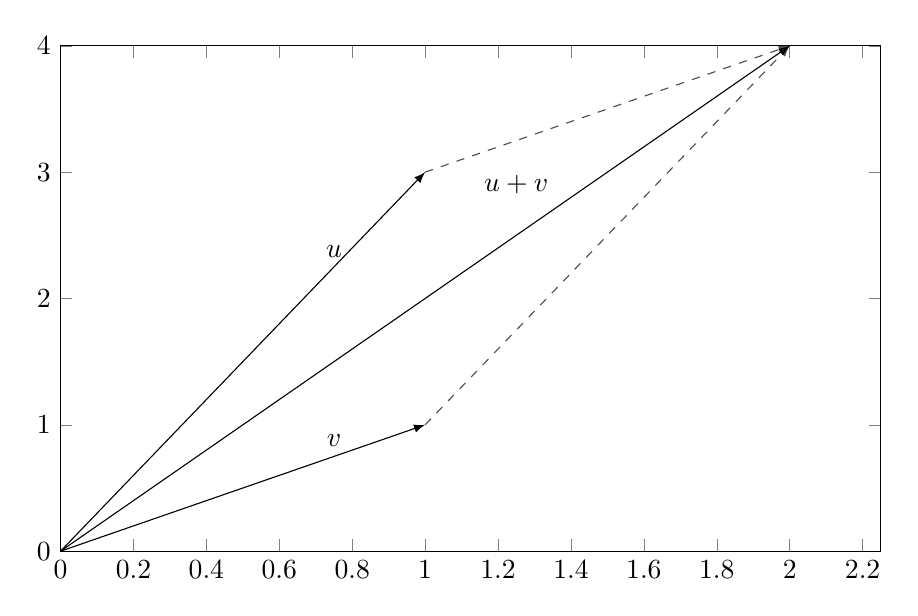
\begin{tikzpicture}
    \begin{axis}[name=plot1
      %,title=
      ,width=12cm
      ,height=8cm
      ,ymin=0
      ,ymax=4
      ,xmin=0
      ,xmax=2.25
      ,domain=0:2.25
      %,ylabel=$y$
      %,xlabel=$x$
    ]
    \draw [->, >=latex] (axis cs:0, 0) -- (axis cs:1, 3) ;
    \draw [->, >=latex] (axis cs:0, 0) -- (axis cs:1, 1) ;
    \draw [->, >=latex] (axis cs:0, 0) -- (axis cs:2, 4) ;
    \draw [->, >=latex, dashed, opacity=0.7] (axis cs:1, 3) -- (axis cs:2, 4) ;
    \draw [->, >=latex, dashed, opacity=0.7] (axis cs:1, 1) -- (axis cs:2, 4) ;
    \node[above] at (axis cs:0.75, 2.25) {$u$};
    \node[above] at (axis cs:0.75, 0.75) {$v$};
    \node[above] at (axis cs:1.25, 2.75) {$u + v$};
    \end{axis}
  \end{tikzpicture}
  \caption{Example of a Linear Transformation}
  \label{fig:example_of_a_linear_transformation}
\end{figure}

\begin{theorem}
  Let $V, W$ be vector spaces, $T: V \to W$ a linear transformation, and $\set{v_i}$ a basis for $V$. Then
  \[
    T(v) = \sum^{}_{i} \alpha_i T(v_i)
  \]

  for $v = \sum^{}_{i} \alpha_i v_i$.
\end{theorem}

\begin{proof}
  We have that
  \[
    T(v) = T\left(\sum^{}_{i} \alpha_i v_i\right)
  \]

  We can then proceed by induction, using the properties of a linear transformation we saw above. Since $V$ is a linear space, it has all its  linear combinations. Thus $\alpha_1 v_1 \in V$ and $\sum^{}_{i > 1} \alpha_i v_i \in V$. Applying the definition,
  \[
    T(v)
    =
    T\left(\alpha_1 v_1 + \sum^{}_{i > 1} \alpha_i v_i\right)
    =
    \alpha_1 T\left(v_1\right) + T\left(\sum^{}_{i > 1} \alpha_i v_i\right)
  \]

  Iterating the above:
  \[
    T(v)
    =
    \sum^{}_{i < k}
    \alpha_i T\left(v_i\right)
    +
    T\left(\alpha_k v_k + \sum^{}_{i > k} \alpha_k v_k\right)
    =
    \sum^{}_{i < k}
    \alpha_i T\left(v_i\right)
    +
    \alpha_k T(v_k)
    +
    T\left(\sum^{}_{i > k} \alpha_k v_k\right)
  \]

  Therefore we can simply write
  \[
    T(v) = \sum^{}_{i} \alpha_i T\left(v_i\right)
  \]
\end{proof}

\begin{theorem}
  Any linear transformation $T: V \to W$ can be represented by a matrix.
\end{theorem}

\begin{proof}
  Let $\dim(V) = M \le N$ so $V \subseteq \mathbb{R}^N$. A matrix $A$ is a collection of vectors $\set{a_1, \ldots, a_M}$ with $a_i \in W$. Now consider the standard basis $\set{e_i}$ for $\mathbb{R}^N$ and take the subset of the standard basis that spans $V$. WLOG take these to be the first $M$ elements of the sandard basis. For any vector $x \in V$ we find
  \begin{align*}
    T(x)
    =
    T\left(\sum^{}_{i} x_i e_i \right)
    =
    \sum^{}_{i} x_i T\left(e_i \right)
  \end{align*}

  Let $a_i \equiv T(e_i)$ and we can see that
  \begin{align*}
    T(x) = Ax = \sum^{}_{i} a_i x_i
  \end{align*}

  Hence $T: V \to W$ can be equivalently represented by $A = [a_1 ~~ \cdots ~~ a_M]$ with $a_i \in W$.
\end{proof}

\begin{example}
  Consider the following operation
  \[
    \left[\begin{matrix}
        1 & 2 & 3 \\
        4 & 5 & 6
    \end{matrix}\right]
    \left[\begin{matrix}
        4 \\ 6 \\ 8
    \end{matrix}\right]
    =
    4 \left[\begin{matrix}
        1 \\
        4
    \end{matrix}\right]
    +
    6 \left[\begin{matrix}
        2 \\
        5
    \end{matrix}\right]
    +
    8 \left[\begin{matrix}
        3 \\
        6
    \end{matrix}\right]
  \]

  Which we express as a linear transform
  \[
    T(e_1) = \left[\begin{matrix}
        1 \\
        4
    \end{matrix}\right]
    \quad\quad
    T(e_2) =  \left[\begin{matrix}
        2 \\
        5
    \end{matrix}\right]
    \quad\quad
    T(e_3) = \left[\begin{matrix}
        3 \\
        6
    \end{matrix}\right]
  \]

  That is,
  \[
    T\left(\begin{matrix}
    4 \\ 6 \\ 8
    \end{matrix}\right)
    =
    4 T(e_1)
    + 6 T(e_2)
    + 8 T(e_3)
  \]
\end{example}

In general we can define matrix multiplication as linear operations on vector spaces:
\[
  A B = A [b_1 \ldots b_N] = \left[A b_1 \ldots Ab_N\right]
\]

Some properties of \keyword{matrix multiplication}:
\begin{enumerate}
  \item \keyword{Associativity}: $(AB)C = A(BC)$
  \item \keyword{Distributivity}: $A(B + C) = AB + AC$
\end{enumerate}

However, in general \textbf{\textit{matrix multiplication is not commutative}}. That is, $AB \ne BA$ in general (in fact, $BA$ may not even be well-defined). Although matrix addition \textit{is} commutative: $A + B = B + A$.

\subsubsection{Matrix Inverse, Rank, and Determinant}
\label{ssub:matrix_inverse_rank_and_determinant}

\begin{definition}
  The vector space spanned by the columns of a matrix $A$ is the \keyword{column space} of $A$. The \keyword{rank} of a matrix, $\rank(A)$, is the dimension of the column space (the maximum number of linearly independent columns).\footnote{It turns out that the row-rank of a matrix, the maximum number of linearly independent rows, is the same as the column-rank of a matrix. Hence  we can just  talk about the rank without clarifying row or column.} A square matrix $N \times N$ is called \keyword{full-rank} if $\rank(A) = N$ and \keyword{rank-deficient} if $\rank(A) < N$.
\end{definition}

\begin{definition}
  A $N \times N$ matrix $A$ is called \keyword{diagonal} if all its non-diagonal entries are $0$.
\end{definition}

\begin{definition}
  The \keyword{identity matrix} is an $N \times N$ diagonal matrix with all diagonal entries equal to $1$ (and non-diagonal entries equal to $0$). For any $N \times N$ matrix $A$, $AI = IA = A$.
  \[
    I = \left[\begin{matrix}
        1    & 0      & 0 &        & 0      \\
        0    & 1      & 0 & \cdots & 0      \\
        0    & 0      & 1 &        & 0      \\
             & \vdots &   & \ddots & \vdots \\
        0    & 0      & 0 & \cdots & 1      \\
    \end{matrix}\right]
  \]
\end{definition}

\begin{definition}
  The $N \times N$ matrix $A$ is said to be \keyword{left invertible} if $\exists C_L$ s.t. $C_L A = I$ the identity. We say it is \keyword{right invertible} if $\exists C_R$ s.t. $A C_R = I$. If $A$ is left and right invertible with $C_L = C_R$, we say that $A$ is \keyword{invertible}, and we denote $C_R = C_L = A^{-1}$ the \keyword{inverse} of $A$.\footnote{The left and right inverses are the same for a square matrix if either exist, but this is a result, not an assumption. Further, note you can define the left and right inverses for non-square matrices, but such matrices needn't be invertible as only one of $C_L$ or $C_R$ might exist.}
\end{definition}

\begin{definition}
  If $A$ is not invertible, we say that $A$ is \keyword{singular}.
\end{definition}

\begin{theorem}
  Let $A$ be a $N \times N$ matrix. $A$ is invertible $\iff \rank(A) = N$.
\end{theorem}

Some other properties of the rank:
\begin{itemize}[label=$\bullet$]
  \item $\rank(A) = \rank(A^T) = \rank(A A^T) = \rank(A^T A)$.
  \item $\rank(AB) \le \min\Fset{\rank(A), \rank(B)}$.
  \item $\rank(CAB) = \rank(A)$ if $C, B$ are non-singular.
\end{itemize}

\begin{example}
  Can we find the inverse of the matrix
  \[
    B = \left[\begin{matrix}
      2 & 1 \\ 1 & 1
    \end{matrix}\right]
  \]

  using elementary row operations?
  \begin{equation}
    \begin{array}{rl}
      \left[
      \begin{matrix}
        2 & 1 \\
        1 & 1
      \end{matrix}
      \right.
      & \to
      \left.
      \begin{matrix}
        1 & 0 \\
        0 & 1
      \end{matrix}
      \right]
      \\[24pt]
      \left[
      \begin{matrix}
        1 & 1/2 \\
        1 & 1
      \end{matrix}
      \right.
      & \to
      \left.
      \begin{matrix}
        1/2 & 0 \\
        0 & 1
      \end{matrix}
      \right]
      \\[24pt]
      \left[
      \begin{matrix}
        1 & 1/2 \\
        0 & -1/2
      \end{matrix}
      \right.
      & \to
      \left.
      \begin{matrix}
        1/2 & 0 \\
        1/2 & -1
      \end{matrix}
      \right]
      \\[24pt]
      \left[
      \begin{matrix}
        1 & 0 \\
        0 & -1/2
      \end{matrix}
      \right.
      & \to
      \left.
      \begin{matrix}
        1 & -1 \\
        1/2 & -1
      \end{matrix}
      \right]
      \\[24pt]
      \left[
      \begin{matrix}
        1 & 0 \\
        0 & 1
      \end{matrix}
      \right.
      & \to
      \left.
      \begin{matrix}
        1 & -1 \\
        -1 & 2
      \end{matrix}
      \right]
    \end{array}
    \nonumber
  \end{equation}

  The steps here were:
  \begin{enumerate}
    \item Multiply the first row by $1/2$.

    \item Multiply the second row by $-1$ and add the first row to the second row.

    \item Add the  second row to the first row.

    \item Multiply the second row by $-2$.
  \end{enumerate}

  In general, however, we have a shortcut for $2 \times 2$ matrices:
  \[
    B = \left[\begin{matrix}
      a & b \\ c & d
    \end{matrix}\right]
    \quad\quad
    B^{-1}
    =
    \dfrac{1}{ad - bc}
    \left[\begin{matrix}
      d & -b \\ -c & a
    \end{matrix}\right]
    \quad\quad
  \]

  You can check this formula gives exactly what we found using row operations.
\end{example}

\begin{definition}
  The \keyword{determinant} of  a $N \times N$ square matrix $A$ is
  \[
    \det(A) = \sum^{N}_{j = 1} (-1)^{i + j} a_{ij} \det(A_{-i, -j})
  \]

  with $i$ any fixed row of $A$ (i.e. the same $i$ for every $j$).
\end{definition}

Consider this picture:
\begin{figure}[H]
  \centering
  \begin{tikzpicture}
    \begin{axis}[name=plot1
      %,title=
      ,width=12cm
      ,height=8cm
      ,ymin=0
      ,ymax=4
      ,xmin=0
      ,xmax=2.25
      ,domain=0:2.25
      %,ylabel=$y$
      %,xlabel=$x$
    ]
    \draw [->, >=latex] (axis cs:0, 0) -- (axis cs:1, 3) ;
    \draw [->, >=latex] (axis cs:0, 0) -- (axis cs:1, 1) ;
    \draw [->, >=latex] (axis cs:0, 0) -- (axis cs:2, 4) ;
    \draw [->, >=latex, dashed, opacity=0.7] (axis cs:1, 3) -- (axis cs:2, 4) ;
    \draw [->, >=latex, dashed, opacity=0.7] (axis cs:1, 1) -- (axis cs:2, 4) ;
    \node[above] at (axis cs:0.75, 2.25) {$v_1$};
    \node[above] at (axis cs:0.75, 0.75) {$v_2$};
    \node[above] at (axis cs:1.25, 2.75) {$v_1 + v_2$};
    \draw [-, opacity=0, name path = A] (axis cs:0, 0) -- (axis cs:1, 3) --  (axis cs:2, 4);
    \draw [-, opacity=0, name path = B] (axis cs:0, 0) -- (axis cs:1, 1) --  (axis cs:2, 4);
    \addplot[color=shadecolor, opacity=0.5] fill between[of=A and B];
    \end{axis}
  \end{tikzpicture}
\end{figure}

The set
\[
  \Fset{v: v = \sum^{N}_{i = 1} t_i v_i \quad t_i \in [0, 1]}
\]

will give the parallelogram, and the determinant of $V = [v_1 \cdots v_N]$ will be be the area of the parallelogram. (Rather, the absolute value of the determinant; if the determinant is negative that just says something about the direction of the vectors, but the intuition remains.) Some properties of the determinant:
\begin{itemize}[label=$\bullet$]
  \item $\det(AB) = \det(A) \det(B)$.
  \item $\det(A) = \prod_{i} a_{ii}$ if $A$ is diagonal.
  \item $\det(I) = 1$.
  \item $\det(\alpha A) = \alpha^N \det(A)$ for any $\alpha \in \mathbb{R}$.
  \item $\det(A^{-1}) = \det(A)^{-1}$.
\end{itemize}

Another point to make about the determinant is that it is related to the $\rank$, that is, whether the columns (or rows) of a square matrix $A$ are linearly independent.
\begin{enumerate}
  \item If $A$ has a column of row that is all $0$, then $\det(A) = 0$.

    To see this, note that from the formula of the determinant, if we have a row or column of all $0$s, then each element of the sum will eventually be multiplied by $0$, and the entire term will be $0$. Alternatively, if one of the ``sides'' of the parallelogram is between the origin and the origin, the area will be $0$.

  \item If $A$ has two columns or rows that are equal, then $\det(A) = 0$.

    If two columns of $A$ are equal, WLOG let them be the first two columns, consider the matrix $P$ with all diagonal entries equal to $1$ and all but one non-diagonal entries equal to $0$. Let $P_{21} = -1$. That is,
    \begin{align*}
      P
      &
      =
      \begin{bmatrix}
        1      & 0 & 0 & \cdots & 0 \\
        -1     & 1 & 0 & \cdots & 0 \\
        0      & 0 & 1 &        & \vdots \\
        \vdots &   &   & \ddots &   \\
        0      &   &   &        & 0
      \end{bmatrix}
    \end{align*}

    What is $A P$? In this case, with $A = [a_1 ~~ a_2 ~~ \cdots ~~ a_N]$, we have
    \begin{align*}
      A P
      =
      \begin{bmatrix}
        a_1 - a_2 & a_2 & \cdots & a_N
      \end{bmatrix}
      =
      \begin{bmatrix}
        0 & a_2 & \cdots & a_N
      \end{bmatrix}
    \end{align*}

    with the first column equal to $0$ since we assumed the first two columns were equal. Finally, we found in the previous bullet that if a column was all $0$s then the determinant was $0$. Hence
    \begin{align*}
      0
      =
      \det(A P)
      =
      \det(A) \det(P)
      \implies
      \det(A) = 0 \quad\text{or}\quad \det(P) = 0
    \end{align*}

    Note $\det(P) = 1$, so it must be that $\det(A) = 0$.

  \item If $A$ has a columns is a multiple of another column, then $\det(A) = 0$.

    Again WLOG suppose these are the first two columns and let $A$ be as above. If $a_1 = \alpha a_2$ then we can define $P$ almost identically, except $P_{21} = - \alpha$. That is,
    \begin{align*}
      P
      &
      =
      \begin{bmatrix}
        1      & 0 & 0 & \cdots & 0 \\
        -\alpha& 1 & 0 & \cdots & 0 \\
        0      & 0 & 1 &        & \vdots \\
        \vdots &   &   & \ddots &   \\
        0      &   &   &        & 0
      \end{bmatrix}
    \end{align*}

    And again we have $A P = [a_1 - \alpha a_2 ~~ a_2 ~~ \cdots ~~ a_N] = [0 ~~ a_2 ~~ \cdots ~~ a_N]$. Hence $\det(A P) = \det(A) \det(P) = 0$, but again we have $\det(P) = 1$, so $\det(A) = 0$.

  \item If $A$ has a columns or rows that are linearly dependent, then $\det(A) = 0$.

    This is really the point we wanted to make: A determinant of $0$ is tied to the linear dependence of the columns of $A$. This follows from the work we did above: In this case, $\exists \set{\alpha_i}$ s.t. $\alpha_i \ne 0$ for some $i$ s.t.
    \begin{align*}
      a_j = \sum^{}_{i \ne j} \alpha_i a_i
    \end{align*}

    for some $j$. WLOG let $j = 1$, and the matrix $P$ becomes
    \begin{align*}
      P
      &
      =
      \begin{bmatrix}
        1         & 0 & 0 & \cdots & 0 \\
        -\alpha_2 & 1 & 0 & \cdots & 0 \\
        -\alpha_3 & 0 & 1 &        & \vdots \\
        \vdots    &   &   & \ddots & \\
        -\alpha_N &   &   &        & 0
      \end{bmatrix}
    \end{align*}

    So that
    \begin{align*}
      A P
      =
      \begin{bmatrix}
        a_1 - \alpha_2 a_2 - \alpha_3 a_3 \ldots & a_2 & \cdots & a_N
      \end{bmatrix}
      =
      \begin{bmatrix}
        a_1 - \sum^{}_{i \ne  1} \alpha_i a_i & a_2 & \cdots & a_N
      \end{bmatrix}
      =
      \begin{bmatrix}
        0 & a_2 & \cdots & a_N
      \end{bmatrix}
    \end{align*}

    So, one last time, $\det(A P) = \det(A) \det(P) = 0$ and $\det(P) = 1$ implies $\det(A) = 0$.
\end{enumerate}

\begin{theorem}
  $A$ is rank-deficient $\iff \det(A) = 0$.. Equivalently, $A$ is non-invertible $\iff \det(A) = 0$.
\end{theorem}

\begin{definition}
  For a $N \times N$ matrix $A$, the $M_{ij}$ \keyword{minor} is the \textit{determinant} of the $(N - 1) \times (N - 1)$ sub-matrix obtained by deleting the $i$th row and $j$th column of $A$.
\end{definition}

\begin{definition}
  The $i, j$ \keyword{cofactor} of the square $N \times N$ matrix $A$ is given by
  \[
    C_{ij} = (-1)^{i + j} M_{ij}
  \]

  Note one way to write the determinant is as $\det(A) = \sum^{N}_{j = 1} a_{ij} C_{ij}$ for any given $i$.
\end{definition}

\begin{definition}
  The \keyword{adjoint} of an $N \times N$ matrix $A$ is given by
  \[
    \adj(A) = \left[\begin{matrix}
        C_{11} & C_{12} & \cdots & C_{1N} \\
        \vdots &        & \ddots & C_{1N} \\
        C_{N1} & C_{N2} & \cdots & C_{NN}
    \end{matrix}\right]
  \]

  Note the above is a matrix of scalars, since $C_{ij}$ is the product of a determinant, which is a scalar, and $(-1)^{i + j}$, which is a scalar as well.
\end{definition}

\begin{theorem}
  If $A$ is a non-singular $N \times N$ matrix then
  \[
    A^{-1} = \dfrac{1}{\det(A)} \adj(A)
  \]
\end{theorem}

For instance, for a $2 \times 2$ matrix we have
\[
  B = \left[\begin{matrix}
      a & b \\ c & d
  \end{matrix}\right]
\]

Applying the theorem,
\[
  B^{-1}
  =
  \dfrac{1}{\det(B)}
  \left[\begin{matrix}
      C_{11} & C_{12} \\
      C_{21} & C_{22}
  \end{matrix}\right]
  =
  \dfrac{1}{ad - bc}
  \left[\begin{matrix}
      d & -b \\ -c & a
  \end{matrix}\right]
\]

\begin{theorem}[Cramer's Rule]
  Let $A$ be a $N \times N$ non-singular matrix s.t. $A x = b$. Then
  \[
    x_i = \dfrac{\det(\widetilde{A}_i)}{\det(A)}
  \]

  for
  \[
    \widetilde{A}_i = \left[\begin{matrix}
        a_1 & \cdots & a_{i - 1} & b & a_{i + 1} & \cdots & a_N
    \end{matrix}\right]
  \]

  That is, the matrix obtained by replacing the $i$th column of $A$ with $b$.
\end{theorem}

\begin{definition}
  The \keyword{trace} of an $N \times N$ matrix $A$ is the sum of its diagonal elements,
  \[
    tr(A) = \sum^{N}_{i = 1} a_{ii}
  \]
\end{definition}

Some properties of the trace:
\begin{itemize}[label=$\bullet$]
  \item $\trace(A + B) = \trace(A) + \trace(B)$
  \item $\trace(A B) = \trace(BA)$ if both products exist.
  \item $\trace(\alpha A) = \alpha \trace(A)$ for  any $\alpha \in \mathbb{R}$.
\end{itemize}

An example which comes up in econometrics is that for any $N \times K$ matrix $X$ s.t. $\left(X^T X\right)^{-1}$ exists, we have
\[
  \trace\left(\underbrace{X}_{A} \overbrace{(X^T X)^{-1} X^T}^{B}\right)
  =
  \trace((X^T X)^{-1} X^T X)
  =
  \trace(I_{K \times K})
  =
  K
\]

Further,
\[
  \trace\left(I_{N \times N} - X (X^T X)^{-1} X^T\right)
  =
  \trace\left(I_{N \times N}) - \trace(X (X^T X)^{-1} X^T\right)
  =
  N - K
\]

\subsubsection{Eigenvalues and Eigenvectors}
\label{ssub:eigenvalues_and_eigenvectors}

Take
\[
  T(v) =
  \left[\begin{matrix}
    3 & 0 \\ 0 & -1
  \end{matrix}\right]
  \left[\begin{matrix}
    v_1 \\ v_2
  \end{matrix}\right]
\]

\begin{figure}[!ht]
  \centering
  \begin{tikzpicture}
    \begin{axis}[name=plot1
      %,title=
      ,width=12cm
      ,height=8cm
      ,ymin=-3
      ,ymax=3
      ,xmin=0
      ,xmax=6
      ,domain=0:6
      %,ylabel=$y$
      %,xlabel=$x$
    ]
    \draw [->, >=latex] (axis cs:0, 0) -- (axis cs:1.5, 2);
    \draw [->, >=latex] (axis cs:0, 0) -- (axis cs:4.5, -2);
    \draw [->, >=latex] (axis cs:1.5, 1.75) to[bend left=15] (axis cs:4.25, -1.75);
    \node[above] at (axis cs:1.5, 2) {$v = (v_1, v_2)$};
    \node[below] at (axis cs:4.5, -2) {$T(v) = (3v_1, -v_2)$};
    \end{axis}
  \end{tikzpicture}
  \caption{Visualization of a Transformation}
  \label{fig:visualization_of_a_transformation}
\end{figure}

Note that for the standard basis,
\[
  \left[\begin{matrix}
    3 & 0 \\ 0 & -1
  \end{matrix}\right]
  e_1
  =
  3e_1
  \quad\quad
  \left[\begin{matrix}
    3 & 0 \\ 0 & -1
  \end{matrix}\right]
  e_2
  =
  -e_2
\]

For this particular example, we can see the standard basis is exactly scaled by $3$ and $-1$.
\begin{definition}
  Let $A$ be a $N \times N$ square matrix. The $N \times 1$ vector $v \ne 0$ is an \keyword{eigenvector} (or characteristic vector) of $A$ with corresponding \keyword{eigenvalue} or (characteristic root) $\lambda$ if
  \[
    A v = \lambda v
  \]
\end{definition}

In general we want to find a basis $\set{v_i}$ of (the column space of) $A$ s.t.
\[
  Av_i = \lambda_i v_i
\]

that is, a basis of eigenvectors. Note that
\[
  Av = \lambda v
  \iff
  (A - \lambda I) v = 0
\]

This means that for any $v \ne 0$, we have that
\[
  p(\lambda) \equiv \det(A - \lambda I) = 0
\]

$p(\lambda)$ is called the \keyword{characteristic polynomial} of $A$. (Recall that a matrix has a zero determinant if it is singular; in this case if$(A - \lambda I)v = 0$ for any non-zero vector then the columns of $A - \lambda I$ are not linearly independent, and thus the matrix is singular and has a zero determinant.)

\begin{example}\label{example:lecture6_eigen_example}
  Consider
  \[
    A = \left[\begin{matrix}
        1 & 2 \\ 2 & 1
    \end{matrix}\right]
    \quad\quad
    \det
    \left[\begin{matrix}
        1 - \lambda & 2 \\ 2 & 1 - \lambda
    \end{matrix}\right]
    = 0
    \iff
    (1 - \lambda)^2 - 4 = 0
    \iff
    (\lambda + 1)(\lambda - 3) = 0
  \]

  Hence $\lambda = \set{-1, 3}$. These are the \keyword{eigenvalues}. Now we find the \keyword{eigenvectors}. For $\lambda = -1$
  \[
    (A - \lambda I)v = 0
    \iff
    \left[\begin{matrix}
        2 & 2 \\ 2 & 2
    \end{matrix}\right] v = 0
  \]

  Which gives that $v$ must be s.t. $v_1 = -v_2$. For $\lambda = 3$
  \[
    (A - \lambda I)v = 0
    \iff
    \left[\begin{matrix}
        -2 & 2 \\ 2 & -2
    \end{matrix}\right] v = 0
  \]

  Which gives that $v$ must be s.t. $v_1 = v_2$. It is often useful for the norm of the basis to be $1$. Hence the eigenvectors are given by
  \[
    v =
    \dfrac{1}{\sqrt{2}}
    \left[\begin{matrix}
      1 \\ -1
    \end{matrix}\right]
    \quad\text{and}\quad
    u =
    \dfrac{1}{\sqrt{2}}
    \left[\begin{matrix}
      1 \\ 1
    \end{matrix}\right]
  \]

  Note that we can express the above as a system:
  \begin{align*}
    A P
    =
    P \Lambda
  \end{align*}

  where
  \begin{align*}
    P = \begin{bmatrix}
      v & u
    \end{bmatrix}
    =
    \begin{bmatrix}
      \dfrac{1}{\sqrt{2}} & \dfrac{1}{\sqrt{2}} \\
      - \dfrac{1}{\sqrt{2}} & \dfrac{1}{\sqrt{2}}
    \end{bmatrix}
    \quad\quad
    \Lambda = \begin{bmatrix}
      -1 & 0 \\
      0 & 3
    \end{bmatrix}
  \end{align*}

  In this case, note $v^T u = 0$ and $v^T v = u^T u = 1$. Hence
  \begin{align*}
    P^T P
    =
    \begin{bmatrix}
      v^T \\ u^T
    \end{bmatrix}
    \begin{bmatrix}
      v & u
    \end{bmatrix}
    =
    \begin{bmatrix}
      v^T v & v^T u \\
      u^T v & u^T u
    \end{bmatrix}
    =
    \begin{bmatrix}
      1 & 0 \\
      0 & 1
    \end{bmatrix}
  \end{align*}

  and if we pre-multiply the eigen-system by $P^T$ we get
  \begin{align*}
    P^T A P = \Lambda
  \end{align*}
\end{example}

\begin{definition}
  $A$ an $N \times N$ matrix is \keyword{diagonalizable} if $\exists P$ and diagonal matrix $\Lambda$ s.t.
  \[
    P^{-1} A P = \Lambda
  \]

  Note we can equivalently write $A = P \Lambda P^{-1}$.
\end{definition}

It will be useful to note if $A$ is diagonalizable
\begin{itemize}[label=$\bullet$]
  \item $A^m$ for any $m \in \mathbb{N}$ can computed as $P \Lambda^m P^{-1}$.
    \begin{align*}
      A^m
      =
      A
      \times \ldots \times
      A
      =
      P \Lambda P^{-1}
      \times \ldots \times
      P \Lambda \times \ldots \times \Lambda P^{-1}
      =
      P \Lambda^m P^{-1}
    \end{align*}

    since each of the $P^{-1} P$ cancel and $\Lambda \times \Lambda = \Lambda^2$ and so on.

  \item $A^{1/m}$ for any $m \in \mathbb{N}$ can computed as $P \Lambda^{1/m} P^{-1}$.
    \begin{align*}
      \left(
        P \Lambda^{1/m} P^{-1}
      \right)^m
      =
      P \Lambda^{1/m} P^{-1}
      \times \ldots \times
      P \Lambda^{1/m} P^{-1}
      =
      P \Lambda^{1/m} \times \ldots \times \Lambda^{1/m} P^{-1}
      =
      P \Lambda P^{-1}
      =
      A
    \end{align*}

  \item If $\Lambda$ is invertible, then $A^{-m}$ for any $m \in \mathbb{N}$ can computed as $P \Lambda^{-m} P^{-1}$.
    \begin{align*}
      A^{-m}
      =
      \left(
        A^m
      \right)^{-1}
      =
      \left(
        P \Lambda^m P^{-1}
      \right)^{-1}
      =
      P \Lambda^{-m} P^{-1}
    \end{align*}

    and we can check
    \begin{align*}
      A^m A^{-m}
      =
      P \Lambda^{m} P^{-1} P \Lambda^{-m} P^{-1}
      =
      P \Lambda^{m} \Lambda^{-m} P^{-1}
      =
      P P^{-1}
      =
      I
    \end{align*}

  \item Similarly, if $\Lambda$ is invertible $A^{-1/m}$ for any $m \in \mathbb{N}$ can computed as $P \Lambda^{-1/m} P^{-1}$.

  \item Let $q \in \mathbb{Q}$ (so $q = m/n$ for $m, n \in \mathbb{Z}$). Then $A^q = (A^m)^{1/n}$ is $P (\Lambda^m)^{1/n} P^{-1} = P \Lambda^q P^{-1}$.

  \item Finally, $A^r = P \Lambda^r P^{-1}$ for any $r \ge 0$ (if in addition $\Lambda$ is invertible, this holds for any $r \in \mathbb{R}$).
\end{itemize}

\begin{claim}
  If $A$ is diagonalizable then $P$ is a matrix of eigenvectors and $\Lambda$ is a matrix of eigenvalues.
\end{claim}

\begin{proof}
  If $A$ is  diagonalizable then
  \[
    A P = P \Lambda
  \]

  Since the $k$th column of $P$ is s.t. $A v_k = \lambda_k v_k$ we can see $v_k$ is an eigenvector and $\lambda_k$ an eigenvalue.
\end{proof}

\begin{theorem}
  Let $A$ be a $N \times N$ matrix with eigenvalues $\lambda_1, \ldots, \lambda_N$.
  \begin{itemize}[label=$\bullet$]
    \item $\trace(A) = \sum^{N}_{i = 1} \lambda_i$
    \item $\det(A) = \prod_{i = 1}^N \lambda_i$.
  \end{itemize}
\end{theorem}

\begin{proof}
  Let us show this assuming $A$ is diagonalizable.\footnote{
    For the general proof, recall $\lambda_1, \ldots, \lambda_N$ are the roots of the polynomial given by
    \begin{align*}
      \det(A - \lambda I)
      =
      (\lambda_1 - \lambda)
      \times
      (\lambda_2 - \lambda)
      \times
      \ldots
      \times
      (\lambda_N - \lambda)
    \end{align*}

    For the determinant, set $\lambda = 0$ and find $\det(A) = \prod_{i = 1}^N \lambda_i$. For the trace, we need to leverage something known as ``Vieta's formulas.'' The relevant result is that for a polynomial of order $N$, the $N - 1$ coefficient is the sum of the roots of the polynomial (this sounds esoteric, but think about how you learned to expand formulas like $(\lambda_1 - \lambda) (\lambda_2 - \lambda)$; the ``middle'' term is $- (\lambda_1 + \lambda_2)$, and this is just the generalization). If we can show $\trace(A)$ is the $N - 1$ coefficient of the characteristic polynomial we'd be done. To see it, note that $\lambda^{N - 1}$ will only appear if all the diagonal elements are multiplied (any other permutation will give at most a polynomial of order $N - 2$). Hence $\lambda^{N - 1}$ only appears as part of the term
    \begin{align*}
      \prod_{i} (a_{ii} - \lambda)
    \end{align*}

    Here the roots are $a_{ii}$, so the coefficient on $\lambda^{N - 1}$ is $\sum^{}_{i} a_{ii} = \trace(A)$.
  }
  \begin{align*}
    \trace(A)
    &
    = \trace(P^{-1} \Lambda P)
    = \trace(\Lambda P P^{-1})
    = \trace(\Lambda)
    = \sum^{}_{i}  \lambda_i
    \\
    \det(A)
    &
    = \det(P^{-1} \Lambda P)
    = \det(P^{-1}) \det(\Lambda) \det(P)
    = \det(\Lambda)
    = \prod^{}_{i}  \lambda_i
  \end{align*}
\end{proof}

\begin{theorem}
  If $A$ is symmetric then $A$ is diagonalizable and $P$ can be chosen to be orthonormal ($P^{-1} = P^T$ with each column of $P$ equal to a unit vector). This is known as the \keyword{spectral decomposition}.
\end{theorem}

Recall in \Cref{example:lecture6_eigen_example}, the matrix $A$ we considered was symmetric, and we found a diagonalization where $P^{-1} = P^T$. This theorem states that we can do this for any symmetric matrix. Below I present an example for a matrix that is not symmetric.
\begin{remark}
  I am not altogether in the know about linear algebra terminology. I have heard this type of diagonalization be referred to as eigendecomposition, which is intuitive, and as spectral decomposition, as it apparently comes from the spectral theorem. However, a spectre sounds too spooky for this class.
\end{remark}

\begin{theorem}
  Let $A$ be a symmetric $N \times N$ matrix. Then
  \begin{enumerate}
    \item $A$ is PD (ND) $\iff$ $\lambda_i > 0$ ($< 0$) for all eigenvalues $\lambda_i$ of $A$.
    \item $A$ is PSD (NSD) $\iff$ $\lambda_i \ge 0$ ($\le 0$) for all eigenvalues $\lambda_i$ of $A$.
  \end{enumerate}
\end{theorem}

\begin{proof}
  If $A$ is symmetric, then
  \begin{equation}
    v^\prime A v = v^\prime P \Lambda P^T v = u^T \Lambda u
  \end{equation}

  for $u = P^T v$ (since $P$ is non-singular, $u \ne 0$ if $v \ne 0$). Hence the definiteness of $A$ is the same as the definiteness of $\Lambda$. From here we can see that
  \begin{equation}
    u^T \Lambda u = \sum^{N}_{i = 1} \lambda_i u_i^2
  \end{equation}

  where $u_i^2 \ge 0$ (strict for at least one $i$). If $\lambda_i > 0$ for all $i$, $v^\prime A v = \sum^{N}_{i = 1} \lambda_i u_i^2 > 0$, so it is PD. Conversely, if $A$ is PD, we know $v^\prime A v > 0$ for any $v \ne 0$. In particular, it must be true for $v$ equal to each of the columns of $P$. Since the columns of $P$ are orthonormal, for $v = p_i$ the $i$th column of $P$, $C^T p_i = e_i$ the $i$th standard vector (i.e. $1$ in the $i$th entry and $0$ elsewhere). Hence $v^\prime A v = \lambda_i$ when $v = p_i$; since all such quadratic forms are positive, $\lambda_i > 0$. The logic for $< 0$ and ND, $\ge 0$ and PSD, and $\le 0$ and NSD is completely analogous.
\end{proof}

\paragraph{EigenExample}
\label{par:eigenexample}

\[
  A = \left[\begin{matrix}
      1 & 2 \\ -2 & 1
  \end{matrix}\right]
\]

We can find that $\det(A - \lambda I) = 0$ gives
\[
  (1 - \lambda)^2 + 4 = 0
  \quad\quad
  \lambda = \dfrac{2 \pm \sqrt{4 - 4 \cdot 5}}{2}
\]

Hence $\lambda = 1 \pm 2i$. Solving for $v$, we get
\[
  v_1 = (\alpha, \alpha i)
  \\
  v_2 = (\alpha, -\alpha i)
\]

Let $\alpha = 1$. Then
\[
  P = \left[\begin{matrix}
    1 & 1 \\ i & -i
  \end{matrix}\right]
  \quad\quad
  P^{-1} = \left[\begin{matrix}
    -i & -1 \\ -i & 1
  \end{matrix}\right]
\]

Hence
\[
  A =
  \left[\begin{matrix}
    1 & 1 \\ i & -i
  \end{matrix}\right]
  \left[\begin{matrix}
    1 + i & 0 \\ 0 & 1 - i
  \end{matrix}\right]
  \left[\begin{matrix}
    -i & -1 \\ -i & 1
  \end{matrix}\right]
\]

% ---------------------------------------------------------------------
\subsection{Introduction to Ordinary Differential Equations (ODE)}
\label{sub:introduction_to_ordinary_differential_equations_ode_}

\subsubsection{Dynamic Equations}
\label{ssub:dynamic_equations}

The basic idea is that we want to understand how a variable changes over time. If time is continuous (like it is IRL), then we say that
\[
  \dot{y}
  \equiv
  \dfrac{dy}{dt}
\]

In general, we have an $n$th order linear differential equation as
\[
  y^{(n)} + \alpha_{n - 1}(t) y^{(n - 1)} + \ldots + \alpha_0(t) y = f(t)
\]

where $\alpha_{i}(t)$ are constants that depend only on $t$ and $y^{(n)}$ is the $n$th derivative of $y$ with respect to $t$. We say it is \keyword{homogeneous} if $f(t) = 0$.

The equation is called \keyword{autonomous} if $t$ only enters through $y(t)$; that is, $\alpha_i(t) \equiv \alpha_i$. For example,
\[
  \dot{y} = k y
  \iff
  \dot{y} - k y = 0
\]

is an autonomous \textit{and} homogeneous equation. By contrast,
\[
  \dot{y} = t y
  \iff
  \dot{y} - t y = 0
\]

is homogeneous \textit{but not} autonomous.
\begin{example}
  Consider the autonomous and homogeneous system
  \[
    \dot{y} = ky
  \]

  This translates to
  \[
    \dfrac{dy}{dt} = ky
  \]

  which means that
  \[
    \int_{}^{} \dfrac{dy}{dt} \dfrac{1}{y} dt
    =
    \int_{}^{} k dt
    \iff
    \log(y) + C_1 = kt + C_2
  \]

  Let $C_3 \equiv \exp(C_2 - C_1)$, and we have that
  \[
    y = C_3 e^{kt}
  \]

  This equation is not quite defined, since the behavior of $y$ depends on the constant $C_3$. Hence we need some initial conditions to pin down the path of $y$ with respect to $t$. For example,
  \[
    y(0) = 5
    \quad\quad
    5 = C_3 e^{0}
    \implies
    C_3 = 5
    \implies
    y(t) = 5 e^{kt}
  \]
\end{example}

\begin{example}
  Consider the homogeneous but not autonomous system
  \[
    \dot{y} = ty
  \]


  Again,
  \[
    \dfrac{dy}{dt} = ty
  \]

  which means that
  \[
    \int_{}^{} \dfrac{dy}{dt} \dfrac{1}{y} dt
    =
    \int_{}^{} t dt
    \iff
    \log(y) + C_1 = \dfrac{t^2}{2} + C_2
  \]

  Let $C_3 \equiv \exp(C_2 - C_1)$, and we have that
  \[
    y = C_3 e^{\dfrac{t^2}{2}}
  \]

  Note that $y(0) = C_3$. Hence we can write
  \[
    y(t) = y(0) e^{\dfrac{t^2}{2}}
  \]
\end{example}

We will not always use the separation of variables method. In general, if we have an equation of the form
\[
  \dot{y} + p(t) y = q(t)
\]

that will be neither autonomous nor homogeneous. One method to solve this system is to use the \keyword{integrating factor}. Multiply each term by $\exp(\int p(t) dt)$:
\[
  \exp\left\{\int_{}^{} p(t) dt\right\}
  \left(\dot{y} + p(t) y\right)
  =
  \exp\left\{\int_{}^{} p(t) dt\right\}
  q(t)
\]

Why? Because we have that
\[
  \dfrac{d}{dt}
  \left(
    \exp\left\{\int_{}^{} p(t) dt\right\}
    y
  \right)
  =
  \exp\left\{\int_{}^{} p(t) dt\right\} \dot{y}
  +
  \exp\left\{\int_{}^{} p(t) dt\right\} p(t) y
\]

Hence
\[
  \int_{}^{}
  \left[
    \dfrac{d}{dt}
    \left(
      \exp\left\{\int_{}^{} p(t) dt\right\}
      y
    \right)
  \right]
  dt
  =
  \int_{}^{}
  \left[
    \exp\left\{\int_{}^{} p(t) dt\right\}
    q(t)
  \right]
  dt
\]

gives
\[
  y(t)
  =
  \dfrac{
    \int_{}^{}
    \left[
      \exp\left\{\int_{}^{} p(t) dt\right\}
      q(t)
    \right]
    dt
    +
    C
  }{
    \exp\left\{\int_{}^{} p(t) dt\right\}
  }
\]

for some constant $C$. Let's see an example:

\begin{example}
  Consider the system
  \[
    \dot{y} + t^2 y = t^2
  \]

  How to proceed in this case?
  \[
    \dot{y} = ay + b
  \]

  $p(t) = -a$ and $q(t) = b$. The integrating factor is
  \[
    \exp\left\{\int_{}^{} p(t) dt\right\}
    =
    \exp\left\{\int_{}^{} -a dt\right\}
    =
    \exp\left\{-at\right\}
  \]

  Plugging the formula,
  \[
    y(t) =
    \dfrac{
      \int_{}^{}
      \exp\left\{-at\right\} b dt
      + C
    }{
      \exp\left\{-at\right\}
    }
    =
    - \dfrac{b}{a}
    + C \exp\left\{at\right\}
  \]
\end{example}

\subsubsection{Dynamic Systems}
\label{ssub:dynamic_systems}

Consider an equation in discrete time
\[
  y_t = \alpha y_{t - 1} + x_t
\]

An $n$th order \keyword{linear difference} equation is
\[
  y_{t - n}
  + \alpha_{(n - 1)}(t) y_{t - (n - 1)}
  + \ldots
  + \alpha_{0}(t) y_{t}
  =
  f(t)
\]

We say that this is \keyword{homogeneous} if $f(t) = 0$ and \keyword{autonomous} if $\alpha_i(t) \equiv \alpha_i$ do not depend on $t$. The way to solve this is by recursive computation:
\[
  y_t = \dfrac{1}{k} y_{t - 1}
\]

In general,
\[
  y_t
  = \dfrac{1}{k^2} y_{t - 2}
  = \dfrac{1}{k^3} y_{t - 3}
  = \ldots
  = \dfrac{1}{k^t} y_{0}
\]

For example take the $2$nd order homogeneous and autonomous difference equation
\[
  y_{t - 2} + \alpha y_{t - 1} + \beta y_{t} = 0
\]

We assume that $y_t = Ca^t$, and we check against that. So
\[
  Ca^{t - 2}
  + \alpha Ca^{t - 1}
  + \beta Ca^{t}
  = 0
  \iff
  a^{-2}
  + \alpha a^{-1}
  + \beta
  = 0
  \iff
  \beta a^2 + \alpha a + 1 = 0
\]

Hence
\[
  a = \dfrac{-\alpha \pm \sqrt{\alpha^2 - 4\beta}}{2\beta}
\]

Considera first-order \keyword{dynamic system}:
\[
  x_t = A x_{t - 1}
\]

If $A$ is diagonalizable, then
\[
  x_t
  = P^{-1} \Lambda P \left(P^{-1} \Lambda P x_{t - 2}\right)
  = P^{-1} \Lambda^2 P x_{t - 2}
  = \ldots
  = P^{-1} \Lambda^t P x_{0}
\]

Hence the dynamics of the system can be determined by analyzing the matrix of eigenvectors $\Lambda$.
\begin{itemize}[label=$\bullet$]
  \item If all eigenvalues have absolute value $< 1$ then the system is globally stable ($\Lambda^t \to 0$).

  \item If all eigenvalues have absolute value $> 1$ then the system is globally unstable ($\Lambda^t \to \pm \infty$)..
\end{itemize}

In continuous time, consider
\[
  \dot{x} = A x
\]

Again, assuming $A$ id diagonalizable,
\[
  P \dot{x} = \Lambda P x
\]

Let $y = P x$, so $\dot{y} = P \dot{x}$, and we have
\[
  \dot{y} = \Lambda y
\]

with $\Lambda$ diagonal. In this case, the solution is given by
\[
  y = \exp(\Lambda t) C
\]

for some constant vector $C$ and $\exp(\Lambda t)$ denoting the diagonal matrix $\diag{\lambda_1 t, \ldots, \lambda_N t}$. Note
\[
  \dot{y}
  =
  \Lambda
  \underbrace{\exp(\Lambda t) C}_y
  =
  \Lambda y
\]

% % ---------------------------------------------------------------------
% \clearpage
%
% \setcounter{subsection}{0}
% \renewcommand\thesubsection{\Alph{subsection}}
% \titleformat{\subsection}[display]{
%   \Large\bfseries
% }{Appendix \thesubsection. #1}{0pt}{\vspace{-24pt}}
% \renewcommand\thesubsubsection{\Alph{subsection}.\arabic{subsubsection}}
% \crefalias{section}{appendix}
% \crefalias{subsection}{appendix}
%
% \subsection{Linear Algebra in the Abstract}
% \label{sub:appendix_linear_algebra_in_the_abstract}
%
% Only for the very curious, I will exhibit here an entirely formal treatment of linear spaces and build up to the theorem I mentioned wherein we see that any linear space (under a very mild condition; namely that it is finite-dimensional) is equivalent to $\mathbb{R}^N$. Proofs for this appendix are available on request, but again this is just here to show you there is a very abstract and formal way of defining everything, even if it leads to the exact place you would expect (the  real numbers).
%
% \begin{definition}
%   A \keyword{binary operator} on $X$ is a map $f: X \times X \to X$. We denote $f(x, y) \equiv x f y$.
% \end{definition}
%
% \begin{definition}
%   Let $X$ be a non-empty set and $+$ a binary operator. $(X, +)$ is a \keyword{group} if the following hold:
%   \begin{enumerate}
%     \item \keyword{Associativity}: $+(+(x, y), z) = +(x, +(y, z))$; that is, $(x + y) + z = x + (y + z)$.
%
%     \item Existence of an \keyword{additive identity}: $\exists e \in X$ s.t. $e + x = x = x + e$. We denote $e \equiv 0$, i.e. $0 + x = x = x + 0$.
%
%     \item Existence of an \keyword{additive inverse}: $\forall x \in X ~~ \exists y$ s.t. $x + y = y + x = 0$. We denote $y \equiv -x$.
%   \end{enumerate}
% \end{definition}
%
% Note we are using $+$ to denote addition (because, seriously, what else would we use?)
% \begin{definition}
%   A group $(X, +)$ is an \keyword{Abelian group} if the following also holds:
%   \begin{enumerate}[start=4]
%     \item \keyword{Commutativity}: $+(x, y) = +(y, x)$; that is, $x + y = y + x$.
%   \end{enumerate}
% \end{definition}
%
% An easy example of an Abelian group is $\mathbb{R}$ with addition. A more complex example:
% \begin{example}
%   Consider a Rubiks cube and the set of all possible permutations of the faces. This is a group:
%   \begin{itemize}[label=$\bullet$]
%     \item There is an identity element, namely the solved cube.
%
%     \item There is an inverse element: Given any permutation, the set of operations that solves the cube would give the inverse element from the solved cube.
%
%     \item It is associative: Given any sequence of permutations, as long as they are applied in the same sequence, whether we ``group'' any set of operations together doesn't matter.
%   \end{itemize}
%
%   However, this is \textbf{\textit{not}} an Abelian group because operations on the cube are not commutative---order matters.
% \end{example}
%
% \begin{claim}
%   Let $(X, +)$ be a group:
%   \begin{itemize}[label=$\bullet$]
%     \item The identity element is unique.
%
%     \item The inverse element is unique.
%   \end{itemize}
% \end{claim}
%
% \begin{definition}
%   $(X, +, \bcdot)$ is a \keyword{linear space} (or \keyword{vector space}) if $(X, +)$ is an Abelian group and $\bcdot: \mathbb{R} \times X \to X$ satisfies, for any $\alpha, \lambda \in \mathbb{R}$ and $\vec{x}, \vec{y} \in X$,
%   \begin{enumerate}
%     \item \keyword{Associativity}: $\bcdot(\alpha, \bcdot(\lambda, \vec{x})) = \bcdot(\alpha \lambda, \vec{x})$; that is, $\alpha \bcdot (\lambda \bcdot \vec{x}) = (\alpha \lambda) \bcdot \vec{x}$.
%
%     \item \keyword{Distributivity}: In $\mathbb{R}$, $\bcdot(\alpha + \lambda, \vec{x}) = +(\bcdot(\alpha, \vec{x}), \bcdot(\lambda, \vec{x}))$; i.e. $(\alpha + \lambda) \bcdot \vec{x} = \alpha \bcdot \vec{x} + \lambda \bcdot \vec{x}$.
%
%       in $X$, $\bcdot(\lambda, +(\vec{x}, \vec{y})) = +(\bcdot(\lambda, \vec{x}), \bcdot(\lambda, \vec{y}))$; i.e. $\lambda \bcdot (\vec{x} + \vec{y}) = \lambda \bcdot \vec{x} + \lambda \bcdot \vec{y}$.
%
%     \item \keyword{Unit rule}: $\bcdot(1, \vec{x}) = \vec{x}$; that is, $1 \bcdot \vec{x} = \vec{x}$.
%   \end{enumerate}
% \end{definition}
%
% Did you catch the sleight of hand in this definition?\footnote{$\mathbb{R}$ with addition and multiplication as normally defined is what is known as a \keyword{field} (another  example of a field are the rationals, $\mathbb{Q}$). I will not  delve into that here, but the reason linear spaces end up being equivalent fo $\mathbb{R}^N$ is because the field we use to define them is $\mathbb{R}$! This does mean there is a second level of abstraction where if we used some arbitrary field $\mathcal{F}$ then those more abstract linear spaces would be equivalent to $\mathcal{F}^N$.}
% \begin{claim}
%   Let $(X, +, \bcdot)$ be a linear space. Then
%   \begin{itemize}[label=$\bullet$]
%     \item $\lambda \bcdot \vec{0} = \vec{0}$.
%
%     \item $\lambda = 0 \implies \lambda \vec{x} = \vec{0}$.
%
%     \item If $\vec{x} \ne \vec{0}$ then $\lambda \vec{x} = \vec{0} \implies \lambda = 0$.
%
%     \item $-(\lambda \bcdot \vec{x}) = (-\lambda) \bcdot \vec{x}$.
%
%     \item If $\vec{x} \ne  0$ then $\alpha \vec{x} = \beta \vec{x} \iff \alpha = \beta$.
%   \end{itemize}
% \end{claim}
%
% All the above might seem obvious, but try to prove them \textit{only using the definitions} to see why they are not!
% \begin{definition}
%   For any $m \in \mathbb{N}$, a \keyword{linear combination} of $\vec{x}_1, \ldots, \vec{x}_m$ is a vector
%   \begin{align*}
%     \sum^{m}_{i = 1} \lambda_i \vec{x}_i
%   \end{align*}
%
%   with $\lambda_1, \ldots, \lambda_m \in \mathbb{R}$ the \keyword{coefficients} of the linear combination.
% \end{definition}
%
% \begin{theorem}
%   $S$ is a linear space iff it contains all linear combinations of any set of vectors in $S$.
% \end{theorem}
%
% \begin{definition}
%     The set of all linear combinations of finitely many elements of a non-empty set $S$ of is called the \keyword{span} of $S$, defined as the set
%   \begin{align*}
%     \sspan(S)
%     \equiv
%     \bset{
%       \sum^{m}_{i = 1}  \lambda_i \vec{x}_i:
%       m \in \mathbb{N}, (\vec{x}_i, \lambda_i) \in S \times \mathbb{R} ~~ \forall i = 1, \ldots, m
%     }
%   \end{align*}
%
%   By convention, $\sspan(\varnothing) = \set{\vec{0}}$.
% \end{definition}
%
% \begin{definition}
%   A \keyword{basis} for a linear space $X$ is a $\supseteq$-minimal subset of $X$ that spans $X$, i.e. $S$ is a basis for $X$ iff
%   \begin{enumerate}
%     \item $X = \sspan(S)$
%
%     \item $X = \sspan(T) \implies T \cancel\subset S$.
%   \end{enumerate}
% \end{definition}
%
% \begin{definition}
%   If a linear space $X$ has a finite basis then it is finite-dimensional with \keyword{dimension} $\dim(X)$ the cardinality of any of its bases. If $X$ does not have a finite basis, then it is $\infty$-dimensional and $\dim(X) = \infty$.
% \end{definition}
%
% \begin{definition}
%   A subset $S$ of a linear space $X$ is \keyword{linearly dependent} in $X$ if it either equals $\set{\vec{0}}$ or if $\exists \vec{x} \in S$ s.t. $\vec{x}$ can be expressed as a linear combination of finitely many vectors in $S \setminus \set{\vec{x}}$. Any finite set of vectors is called linearly dependent if $\set{x_1, \ldots, x_m}$ is linearly dependent.
% \end{definition}
%
% \begin{definition}
%   A subset $S$ of a linear space $X$ is called \keyword{linearly independent} if no finite subset is linearly dependent. By convention, we say $\varnothing$ is linearly independent.
% \end{definition}
%
% \begin{proposition}\label{proposition:linear_spaces_basis_independent}
%   A subset $S$ of a linear space $X$ is a basis for $X$ iff $S$ is linearly independent and $\sspan(S) = X$.
% \end{proposition}
%
% \begin{corollary}
%   Any two bases of a linear space $X$ have the same cardinality.
% \end{corollary}
%
% \begin{definition}
%   Let $X, Y$ be two linear spaces. A function $L: X \to Y$ is a \keyword{linear operator} or a \keyword{linear transformation} if
%   \begin{align*}
%     L(\alpha \vec{x} + \vec{y})
%     &
%     =
%     \alpha L(\vec{x}) + L(\vec{y})
%     \quad
%     \quad
%     \forall \vec{x}, \vec{y} \in X
%     \quad
%     \text{and}
%     \quad
%     \alpha \in \mathbb{R}
%   \end{align*}
% \end{definition}
%
% \begin{definition}
%   Let $X, Y$ be two linear spaces and $L$ a linear operator $L: X \to Y$. If $L$ is a bijection it is called a \keyword{linear isomorphism} between $X$ and $Y$. If such a bijection exists we say $X$ and $Y$ are \keyword{isomorphic}.
% \end{definition}
%
% \begin{proposition}
%   Two finite-dimensional linear spaces $X, Y$ are isomorphic iff they have the same dimension.
% \end{proposition}
%
% \begin{corollary}
%   Every non-trivial finite-dimensional linear space $X$ (i.e. $X \ne \set{\vec{0}}$) is isomorphic to $\mathbb{R}^{\dim(X)}$.
% \end{corollary}

\clearpage
\printindex

% ---------------------------------------------------------------------
\end{document}
